\documentclass[UTF8,a4paper,11pt]{article}

\usepackage{ctex} 
\usepackage{fancyhdr}
\usepackage{multicol} 
\usepackage{lastpage} 
\usepackage{geometry} 
\usepackage{titlesec} 
\usepackage{mathrsfs}
\usepackage{graphicx}
\usepackage{epstopdf}
\usepackage{ulem}
\usepackage{amsmath}
\usepackage[subfigure,AllowH]{graphfig} 

\geometry{left=3cm,right=3cm,top=2.5cm,bottom=2.5cm}
\renewcommand{\baselinestretch}{1.5}


\title{\huge\heiti《信号与系统》(刘泉、江雪梅主编)复习手册}
\author{AlwaysLoveMisaka}
\date{\today}

\begin{document}
\maketitle
\thispagestyle{empty}
\clearpage

\tableofcontents
\thispagestyle{empty}
\clearpage

\setcounter{page}{1}
\section{前言}
这篇文章是我写的一篇用于复习《信号与系统》的手册,也是我用\LaTeX 写的第一篇文章。通过这篇文章,我打算梳理《信号与系统》(刘泉、江雪梅编)的重点知识。同志们在使用这个手册的时候,最好要结合课本,我也会在文中提及课本第一版(别问我为什么不用最新版,问就是没钱)的内容。

这个手册是在Github上免费提供的,以后也会同步到CSDN上,如果同志们觉得这个好用,可以给我的内容点一个赞。本人Github主页:https://github.com/AlwaysLove Misaka,CSDN主页:https://blog.csdn.net/Communism1848?type=blog。

需要指明的是,本手册并不是考纲。所以,同志们如果发现手册里没有一些考试的内容,请不要来打我,毕竟我就是个垃圾大学生,不是出卷老师。没有写入的内容,部分是我认为不重要或者大家肯定懂,部分是我也没弄明白,部分是我技术有限,很难用\LaTeX 写出来(比如框图,我作为一个\LaTeX 新手是真的不会画)。所以请同志们见谅。

这个手册可以写出来,我首先要感谢的是刘泉、江雪梅两位老师,她们既是教材的编者,也是《信号与系统》这门课我的授课老师。我认为这种情况对于我个人是非常难得的,没有她们对教材的深入讲解,我估计写不出来什么东西。我还要感谢我的父母,他们给我的大学生活提供了经济支持。

另外,我还要感谢御坂美琴,虽然她是一个虚拟的人物,但却是我真实的\sout{老婆}精神支柱。每当想起她,我的生活就充满动力。我好想做御坂大人的狗啊,可是御坂大人说她喜欢的是猫(她是真喜欢猫,如图1),我哭了。我知道既不是狗也不是猫的我为什么要哭的,因为我其实是一只老鼠。我从没奢望御坂大人能喜欢自己,我明白的,所有人都喜欢萌萌的狗狗或者猫猫,没有人会喜欢阴湿带病的老鼠。(此段为作者逆天发病,若感到不适,可以用记号笔涂黑)
\newline
\begin{figure}[htbp]
\centering

\includegraphics[scale=0.2]{cat.jpg}
\caption{御坂妹妹和猫}
\end{figure}

\section{信号与系统的基本概念}
\subsection{信号的分类}
连续时间信号 $f(t)$ 的能量 $E$ 和功率 $P$ 分别定义为
\begin{equation}
E=\lim_{T \to \infty}\int_{-T}^{T} {f^2(t)} \,{\rm d}t
\end{equation}
\begin{equation}
P=\lim_{T \to \infty}\frac{1}{2T}\int_{-T}^{T} {f^2(t)} \,{\rm d}t 
\end{equation}

连续时间信号 $f(k)$ 的能量 $E$ 和功率 $P$ 分别定义为
\begin{equation}
E=\sum_{k=-\infty}^\infty f^2(k)
\end{equation}
\begin{equation}
P=\lim_{N \to \infty}\frac{1}{2N}\sum_{k=-N}^N f^2(k)
\end{equation}

若 $0<E<\infty$ ,且 $P=0$ ,则称此信号为能量信号,即信号能量有限。若 $0<P<\infty$,且 $E$ 趋近于无穷,则称此信号为功率信号,即信号功率有限。

从以上叙述中,我们可以知道,信号可以分成三类:能量信号、功率信号、既不是能量信号也不是功率信号的信号(如 $t\epsilon(t)$ )。一般来说,周期信号都是功率信号。

\subsection{系统的分类}
从数学角度来说,系统可定义为实现某功能的运算。设符号 $T$ 表示系统的运算,将输入信号(又称激励) $e(t)$ 作用于系统,得到输出信号(又称响应) $r(t)$ ,表示为
\begin{equation}
r(t)=T[e(t)] 
\end{equation}

此关系也经常用 $e(t)\to r(t)$来表示。

线性系统是指满足齐次性和叠加性的系统,可以用符号描述为,若 $e_1(t)\to r_1(t)$ , $e_2(t)\to r_2(t)$ ,则
\begin{equation}
T[k_1e_1(t)+k_2e_2(t)]=k_1T[e_1(t)]+k_2T[e_2(t)] 
\end{equation}

其中 $k_1$ 、 $k_2$ 是常数。若不满足上述条件,则为非线性系统。

时不变系统的特性如下
\begin{equation}
r(t-\tau)=T[e(t-\tau)]
\end{equation}

其中 $\tau$ 是常数。若不满足上述条件,则为时变系统。

因果系统是指系统在 $t_0$时刻的响应只取决于 $t\leq t_0$ 时的输入,否则为非因果系统。一般而言,任何物理可实现系统都具有因果性。而理想系统,例如各类理想滤波器,往往具有非因果性。

稳定系统可描述为:若 $\left | e(t) \right |\leq M_1<\infty$ ,则$\left | r(t) \right |\leq M_2<\infty$ 。如不满足上述条件,则为不稳定系统。

本教材主要讨论的是线性时不变系统。

\section{连续时间信号与系统的时域分析}
\subsection{常用典型信号}
抽样信号 $Sa(t)$ 的定义为
\begin{equation}
Sa(t)=\frac{\sin t}{t}
\end{equation}

不难证明
\begin{equation}
\int_{-\infty}^{+\infty} {Sa(t)} \,{\rm d}t=\pi
\end{equation}

单位阶跃信号 $\epsilon(t)$ 的定义为
\begin{equation}
\epsilon(t)=
\begin{cases}
1\quad t>0 \\
0\quad t<0 \\
\end{cases}
\label{pythagorean}
\end{equation}

值得注意的是, $t=0$ 时, $\epsilon(t)$ 未定义。

我们可以用单位阶跃信号表示一些特殊信号,如矩形脉冲信号 $G_{\tau}(t)$ ,它可表示为
\begin{equation}
G_{\tau}(t)=\epsilon(t+\frac{\tau}{2})-\epsilon(t-\frac{\tau}{2}) \label{pythagorean}
\end{equation}

又如符号函数 $sgn(t)$ ,也可以用单位阶跃函数表示为
\begin{equation}
sgn(t)=2\epsilon(t)-1
\end{equation}

单位冲激信号 $\delta(t)$ 的定义为
\begin{equation}
\delta(t)=\lim_{\tau \to 0}\frac{1}{\tau}G_{\tau}(t)
\end{equation}

单位冲激信号有如下特性
\begin{itemize}
\item 抽样(筛选)特性

若 $f(t)$ 连续且有界,则
\begin{equation}
\int_{-\infty}^{+\infty} {f(t)\delta(t-t_0)} \,{\rm d}t=f(t_0)
\end{equation}

\item $\delta(t)$ 为偶函数

\item $\delta(at)=\frac{1}{\left | a \right |}\delta(t)$
\end{itemize}

\subsection{连续时间系统的响应}
可以证明,一个线性时不变(LTI)系统可以用一个线性常系数微分方程表示,如式(15),这里举了一个二阶微分方程的例子。
\begin{equation}
\frac{{\rm d}^2}{{\rm d}t^2}r(t)+a_1\frac{{\rm d}}{{\rm d}t}r(t)+a_0r(t)=b_1\frac{{\rm d}}{{\rm d}t}e(t)+b_0e(t)
\end{equation}

这个方程的完全解由齐次解 $r_h(t)$ 和特解 $r_p(t)$ 组成(高等数学内容,此处复习一下)。齐次解又名自然响应,特解又名受迫响应。

以式(15)的微分方程为例,写出特征方程
\begin{equation}
\lambda^2+a_1\lambda+a_0=0 
\end{equation}

解得特征根 $\lambda_1$ 、 $\lambda_2$ 。

若 $\lambda_1\ne\lambda_2$ ,则方程的齐次解为
\begin{equation}
r_h(t)=C_1e^{\lambda_1t}+C_2e^{\lambda_2t}
\end{equation}

其中, $C_1$ 、 $C_2$ 为常数。若 $\lambda_1=\lambda_2$ ,则方程的齐次解为
\begin{equation}
r_h(t)=(C_1+C_2t)e^{\lambda_1t}
\end{equation}

当激励是常数时,特解也是一个常数。而当激励 $e(t)=e^{\alpha t}$ 时,特解应分三种情况讨论(我只列出来了一部分,完整版可以参考教材p32,因为\LaTeX 的表格,特别是需要合并单元格的表格,实在是太难画了,所以这里没展示出来):
\begin{itemize}
\item 当 $\alpha$ 不等于特征根时, $r_p(t)=Ae^{\alpha t}$ 。
\item 当 $\alpha$ 等于特征单根时, $r_p(t)=(A_1t+A_0)e^{\alpha t}$ 。
\item 当 $\alpha$ 等于2重特征根时, $r_p(t)=(A_2t^2+A_1t+A_0)e^{\alpha t}$ 。
\end{itemize} 

上述 $A$ 、 $A_0$ 、 $A_1$ 、 $A_2$ 皆为常数。需要特别说明的是,特解本身是就是微分方程的一个解。

讲到这里,有些同志可能还是不懂怎么通过这些知识求解响应,下面用一个例子说明。

\textbf{例1:}已知一系统的微分方程为 $\frac{{\rm d}}{{\rm d}t}r(t)+2r(t)=e(t)$ ,初始状态 $r(0_{-})=2$ ,求当激励为 $\epsilon(t)$ 时,系统的全响应。

\textbf{解:}由特征根方程 $\lambda +2=0$ 解得 $\lambda =-2$ ,因此可以得到齐次解(自然响应)
\begin{equation}
r_h(t)=Ce^{-2t}
\notag
\end{equation}

因为激励为常数,因此设特解(受迫响应)
\begin{equation}
r_p(t)=B
\notag
\end{equation}

由于特解本身就是微分方程的解,因此直接代入微分方程,解得 $B=0.5$ ,所以得到全响应
\begin{equation}
r(t)=Ce^{-2t}+\frac{1}{2}
\notag
\end{equation}

将初始状态 $r(0_{-})=2$ 代入全响应公式,解得 $C=1.5$ ,因此得到全响应
\begin{equation}
r(t)=\frac{3}{2}e^{-2t}+\frac{1}{2}\quad(t>0)
\notag
\end{equation}

现在,我们得到了求LTI响应的第一种方法:经典法。其步骤如下:
\begin{itemize}
\item 利用高等数学的传统方法写出带参数的齐次解和通解。
\item 将齐次解代入微分方程解出齐次解。
\item 将初始状态代入全响应解出全响应。
\end{itemize} 

而全响应也有另一种分割方法,即瞬态响应和稳态响应。瞬态响应指 $t\to \infty$ 时响应趋于零的那部分分量,暂态响应指 $t\to \infty$ 时响应不为零零的那部分分量。在例1中,瞬态响应为 $1.5e^{-2t}$ ,稳态响应为 $0.5$ 。需要特别指明的是,瞬态响应和稳态响应是无法直接求解出来的,只能在全响应求出来后进行分割。

\subsection{卷积}
卷积的定义为:
\begin{equation}
f_1(t)*f_2(t)=\int_{-\infty}^{+\infty} {f_1(\tau)f_2(t-\tau)} \,{\rm d}\tau
\end{equation}

卷积的一些性质:
\begin{itemize}
\item 交换律
\begin{equation}
f_1(t)*f_2(t)=f_2(t)*f_1(t)
\end{equation}

\item 分配率
\begin{equation}
f_1(t)*[f_2(t)+f_3(t)]=f_1(t)*f_2(t)+f_1(t)*f_3(t)
\end{equation}

\item 结合率
\begin{equation}
f_1(t)*[f_2(t)*f_3(t)]=[f_1(t)*f_2(t)]*f_3(t)
\end{equation}

\item 时移

若 $f_1(t)*f_2(t)=f(t)$ ,则有 $f_1(t-t_1)*f_2(t-t_2)=f(t-t_1-t_2)$ 。

\end{itemize}

一些常用信号的卷积(我只列出了我认为重要的一部分,更多常用信号的卷积可参考教材p41):
\begin{equation}
f(t)*\delta(t)=f(t)
\end{equation}
\begin{equation}
f(t)*\delta'(t)=f'(t)
\end{equation}
\begin{equation}
f(t)*\epsilon(t)=\int_{-\infty}^{t} {f(\tau)} \,{\rm d}\tau
\end{equation}
\begin{equation}
\frac{{\rm d}f(t)}{{\rm d}t}*\int_{-\infty}^{t} {g(\tau)} \,{\rm d}\tau=f(t)*g(t)
\end{equation}

\subsection{零输入响应与零状态响应}
系统的全响应还可以划分为零输入响应和零状态响应。零输入响应是输入激励为零时,仅由初始状态引起的响应,用 $r_{zi}(t)$ 表示。零状态响应是初始状态为零时,仅由激励引起的响应,用 $r_{zs}(t)$ 表示。

由定义可知,零输入响应的形式与齐次解是相同的,但是零输入响应是通过直接将初始状态代入解得的。

可以证明,一个LTI系统的零状态响应
\begin{equation}
r_{zs}(t)=h(t)*e(t)
\end{equation}

其中, $h(t)$ 是系统的冲激响应。

有了这些信息,我们可以将例1用另一种方法再做一遍。

\textbf{解:}由特征根方程 $\lambda +2=0$ 解得 $\lambda =-2$ ,因此可以得到零输入响应
\begin{equation}
r_{zi}(t)=Ae^{-2t}
\notag
\end{equation}

将初始状态 $r(0_{-})=2$ 代入上式,解得 $A=2$ ,因此解得零输入响应
\begin{equation}
r_{zi}(t)=2e^{-2t}
\notag
\end{equation}

因为零输入响应和齐次解的系数不一样,所以 $h(t)$ 必须带上 $e^{-2t}$ 项。因为 $h(t)$ 需要满足 $\frac{{\rm d}}{{\rm d}t}h(t)+2h(t)=\delta(t)$ ,所以 $h(t)$ 只能有 $e^{-2t}$ 项。因此设
\begin{equation}
h(t)=Be^{-2t}
\notag
\end{equation}

代入微分方程,解得 $B=1$ ,所以零状态响应(这一步使用了式(25))
\begin{equation}
r_{zs}(t)=e^{-2t}*\epsilon(t)=-\frac{1}{2}e^{-2t}+C
\notag
\end{equation}

写出全响应公式
\begin{equation}
r(t)=r_{zi}(t)+r_{zs}(t)=\frac{3}{2}e^{-2t}+C
\notag
\end{equation}

代入初始状态 $r(0_{-})=2$ ,解得全响应
\begin{equation}
r(t)=r_{zi}(t)+r_{zs}(t)=\frac{3}{2}e^{-2t}+\frac{1}{2}
\notag
\end{equation}

由此,我们得到了求LTI响应的第二种方法:时域零输入-零状态法。其步骤如下:
\begin{itemize}
\item 利用特征根写出带参数的零输入响应(其形式与齐次解相同)。
\item 将初始状态代入零输入响应,解得零输入响应。
\item 通过微分方程写出冲激响应的参数形式,然后代入微分方程解得冲激响应。
\item 通过激励与冲激响应的卷积写出零状态响应的参数形式。
\item 将初始状态代入全响应的参数形式,解得全响应。
\end{itemize} 

\section{连续时间信号与系统的频域分析}
\subsection{傅里叶级数}
以高等数学的知识,任何角频率为 $\omega$ 且满足狄里赫利条件的周期函数 $f(t)$ ,可以由三角函数的线性组合来表示。
\begin{equation}
f(t)=\frac{a_0}{2}+\sum_{i=1}^n a_i\cos(i\omega t)+\sum_{i=1}^n b_i\sin(i\omega t)
\end{equation}

式(28)中
\begin{equation}
a_0=\frac{2}{T}\int_{t_0}^{t_0+T} {f(t)} \,{\rm d}t
\end{equation}
\begin{equation}
a_n=\frac{2}{T}\int_{t_0}^{t_0+T} {f(t)\cos(n\omega t)} \,{\rm d}t
\end{equation}
\begin{equation}
b_n=\frac{2}{T}\int_{t_0}^{t_0+T} {f(t)\sin(n\omega t)} \,{\rm d}t
\end{equation}

$\omega$ 为基波频率, $n\omega$ 是 $n$ 次谐波频率。

狄里赫利条件具体如下:
\begin{itemize}
\item 函数绝对可积,即
\begin{equation}
\int_{t_0}^{t_0+T} {\left | f(t) \right |} \,{\rm d}t<\infty
\end{equation}
\item 函数极值数目有限
\item 函数连续或有有限个第一类间断点
\end{itemize} 

函数的对称性与傅里叶级数的关系:
\begin{itemize}
\item 若 $f(t)$ 为偶函数,则 $b_n=0$ 。
\item 若 $f(t)$ 为奇函数,则 $a_0=a_n=0$
\item 满足 $f(t)=-f(t\pm 0.5T)$ 的函数是奇谐函数,其信号波形沿时间轴平移半个周期并相对于时间轴上下翻转后,波形不发生变化。若 $f(t)$ 为奇谐函数,则不含偶次谐波项(包括直流分量)。
\item 满足 $f(t)=f(t\pm 0.5T)$ 的函数是偶谐函数,其信号波形沿时间轴平移半个周期后,波形不发生变化。若 $f(t)$ 为偶谐函数,则不含奇次谐波项(包括基波)。
\end{itemize} 

\subsection{傅里叶变换}
傅里叶变换和反傅里叶变换的定义如下:
\begin{equation}
F(j\omega)=\mathscr{F}[f(t)]=\int_{-\infty}^{\infty} {f(t)e^{-j\omega t}} \,{\rm d}t
\end{equation}
\begin{equation}
f(t)=\mathscr{F}^{-1}[F(j\omega)]=\frac{1}{2\pi}\int_{-\infty}^{\infty} {F(j\omega)e^{-j\omega t}} \,{\rm d}\omega
\end{equation}

也常记为 $f(t)\leftrightarrow F(j\omega)$ 。

可以证明,当 $f(t)\leftrightarrow F(j\omega)$ 时,傅里叶变换有以下性质(此处可参考教材p83):
\begin{itemize}
\item 线性性质(不必多说,可参照此手册p2)
\item 时移性质
\begin{equation}
f(t-t_0)\leftrightarrow F(j\omega)e^{-j\omega t_0}
\end{equation}
\item 频移性质
\begin{equation}
f(t)e^{j\omega_0 t}\leftrightarrow F[j(\omega-\omega_0)]
\end{equation}
\item 尺度变换
\begin{equation}
f(at)\leftrightarrow \frac{1}{\left | a \right |}F(j\frac{\omega}{a})
\end{equation}
\item 对称性
\begin{equation}
F(t)\leftrightarrow 2\pi f(-\omega)
\end{equation}
\item 时域微分
\begin{equation}
\frac{{\rm d}^nf(t)}{{\rm d}t^n}\leftrightarrow (j\omega)^nF(j\omega)
\end{equation}
\item 频域微分
\begin{equation}
(-jt)^nf(t)\leftrightarrow \frac{{\rm d}^nF(j\omega)}{{\rm d}\omega^n}
\end{equation}
\item 时域卷积
\begin{equation}
f_1(t)*f_2(t)\leftrightarrow F_1(j\omega)\cdot F_2(j\omega)
\end{equation}
\item 频域卷积
\begin{equation}
f_1(t)\cdot f_2(t)\leftrightarrow \frac{1}{2\pi}F_1(j\omega)*F_2(j\omega)
\end{equation}
\end{itemize} 

可以证明下列基本函数频谱:
\begin{equation}
\epsilon(t)\leftrightarrow \pi\delta(\omega)+\frac{1}{j\omega}
\end{equation}
\begin{equation}
e^{-\alpha t}\epsilon(t)\leftrightarrow \frac{1}{\alpha+j\omega}
\end{equation}

因为 $\epsilon'(t)=\delta(t)$ ,由式(39),可得
\begin{equation}
\mathscr{F}[\delta(t)]=j\omega(\pi\delta(\omega)+\frac{1}{j\omega})=1
\end{equation}

由式(38)(45),可得
\begin{equation}
1\leftrightarrow 2\pi\delta(\omega)
\end{equation}

因为 $sgn(t)=2\epsilon(t)-1$ ,由线性性质可得
\begin{equation}
\mathscr{F}[sgn(t)]=\mathscr{F}[2\epsilon(t)]-\mathscr{F}[1]=2\pi\delta(\omega)+\frac{2}{j\omega}-2\pi\delta(\omega)=\frac{2}{j\omega}
\end{equation}

通过《复变函数与积分变换》的知识,我们可以知道
\begin{equation}
\cos\omega_0t=\frac{e^{j\omega_0 t}+e^{-j\omega_0 t}}{2}
\end{equation}
\begin{equation}
\sin\omega_0t=\frac{e^{j\omega_0 t}-e^{-j\omega_0 t}}{2j}
\end{equation}

因此由式(36),我们可以得到
\begin{equation}
\mathscr{F}[\cos\omega_0t]=\frac{1}{2}\mathscr{F}[e^{j\omega_0 t}]+\frac{1}{2}\mathscr{F}[e^{-j\omega_0 t}]=\pi[\delta(\omega+\omega_0)+\delta(\omega-\omega_0)]
\end{equation}
\begin{equation}
\mathscr{F}[\sin\omega_0t]=\frac{1}{2j}\mathscr{F}[e^{j\omega_0 t}]-\frac{1}{2j}\mathscr{F}[e^{-j\omega_0 t}]=j\pi[\delta(\omega+\omega_0)-\delta(\omega-\omega_0)]
\end{equation}

由线性性质和时移性质,我们可以得到单位门信号的傅里叶变换。
\begin{equation}
\mathscr{F}[G_{\tau}(t)]=\mathscr{F}[\epsilon(t+\frac{\tau}{2})]-\mathscr{F}[\epsilon(t-\frac{\tau}{2})]=\tau\cdot\frac{e^{j\frac{\omega\tau}{2}}-e^{-j\frac{\omega\tau}{2}}}{2j\cdot\frac{\omega\tau}{2}}=\tau Sa(\frac{\omega\tau}{2})
\end{equation}

利用对称性,将参数 $\tau$ 换成 $\Omega$ 。结合上式,我们可以得到广义抽样信号的傅里叶变换。
\begin{equation}
Sa(t)\leftrightarrow \frac{2\pi}{\Omega}G_{\Omega}(\omega)
\end{equation}

由式(52)(53),我们可以知道,门信号和广义抽样信号是一组傅里叶变换对,这个结论非常重要。

\subsection{连续时间系统的频域分析}
我们知道,系统的零状态响应等于输入信号与系统单位冲激响应的卷积积分。但是,计算两函数的卷积可能是一件非常困难的事。由式(41),我们可以推出
\begin{equation}
R_{zs}(j\omega)=E(j\omega)H(j\omega)
\end{equation}

$H(j\omega)$ 称为系统函数,又称为频率响应函数。有了傅里叶变换这个工具,我们又可以得到一种新的求解LTI系统响应的方法。仍以例1为例,通过p6的方法算出 $h(t)=e^{-2t}$ 后,对单位冲激响应进行傅里叶变换,得
\begin{equation}
H(j\omega)=\frac{1}{2+j\omega}
\notag
\end{equation}

又因为
\begin{equation}
E(j\omega)=\pi\delta(\omega)+\frac{1}{j\omega}
\notag
\end{equation}

所以
\begin{equation}
R_{zs}(j\omega)=E(j\omega)H(j\omega)=\frac{1}{2}\pi\delta(\omega)+\frac{1}{2}(\frac{1}{j\omega}-\frac{1}{2+j\omega})
\notag
\end{equation}

通过傅里叶反变换,解得
\begin{equation}
r_{zs}(t)=\frac{1}{2}-\frac{1}{2}e^{-2t}
\notag
\end{equation}

由此,我们得到了求LTI响应的第三种方法:傅里叶变换法。其步骤如下:
\begin{itemize}
\item 利用特征根写出带参数的零输入响应(其形式与齐次解相同)。
\item 将初始状态代入零输入响应,解得零输入响应。
\item 通过微分方程写出冲激响应的参数形式,然后代入微分方程解得冲激响应。
\item 对冲激响应和输入进行傅里叶变换,相乘即得零状态响应的频域信号。
\item 对零状态响应的频域信号进行傅里叶反变换,得到时域信号,与零输入响应相加即得全响应。
\end{itemize} 

系统函数在线性电路的求解方面还有一些有趣的特性,请看例题:

\textbf{例2:}单位阶跃电压作用于图2所示的电路,求电容器上的电压。

解这道题,我们可以利用电容的伏安特性列出微分方程求解,这样做起来很繁琐。然而,存在这样一个令人欣慰的事实:通过《电路分析》中学到的相量法表示的电容两端电压和电源电压之比就是这个系统的状态方程。而这个电路电容的初始电压为0,因此零状态响应即为全响应。有了这些知识,我们可以很快速地解出这道题。

\textbf{解:}由题意
\begin{equation}
E(j\omega)=\pi\delta(\omega)+\frac{1}{j\omega}
\notag
\end{equation}

然后计算出系统函数
\begin{equation}
H(j\omega)=\frac{\frac{R_2\cdot\frac{1}{j\omega C}}{R_2+\frac{1}{j\omega C}}}{R_1+\frac{R_2\cdot\frac{1}{j\omega C}}{R_2+\frac{1}{j\omega C}}}=\frac{R_2}{R_1+R_2}\cdot\frac{1}{1+j\omega\tau}
\notag
\end{equation}

式中 $\tau=\frac{R_1R_2}{R_1+R_2}C$ ,为电路的时间常数。
\begin{figure}[htbp]
\centering
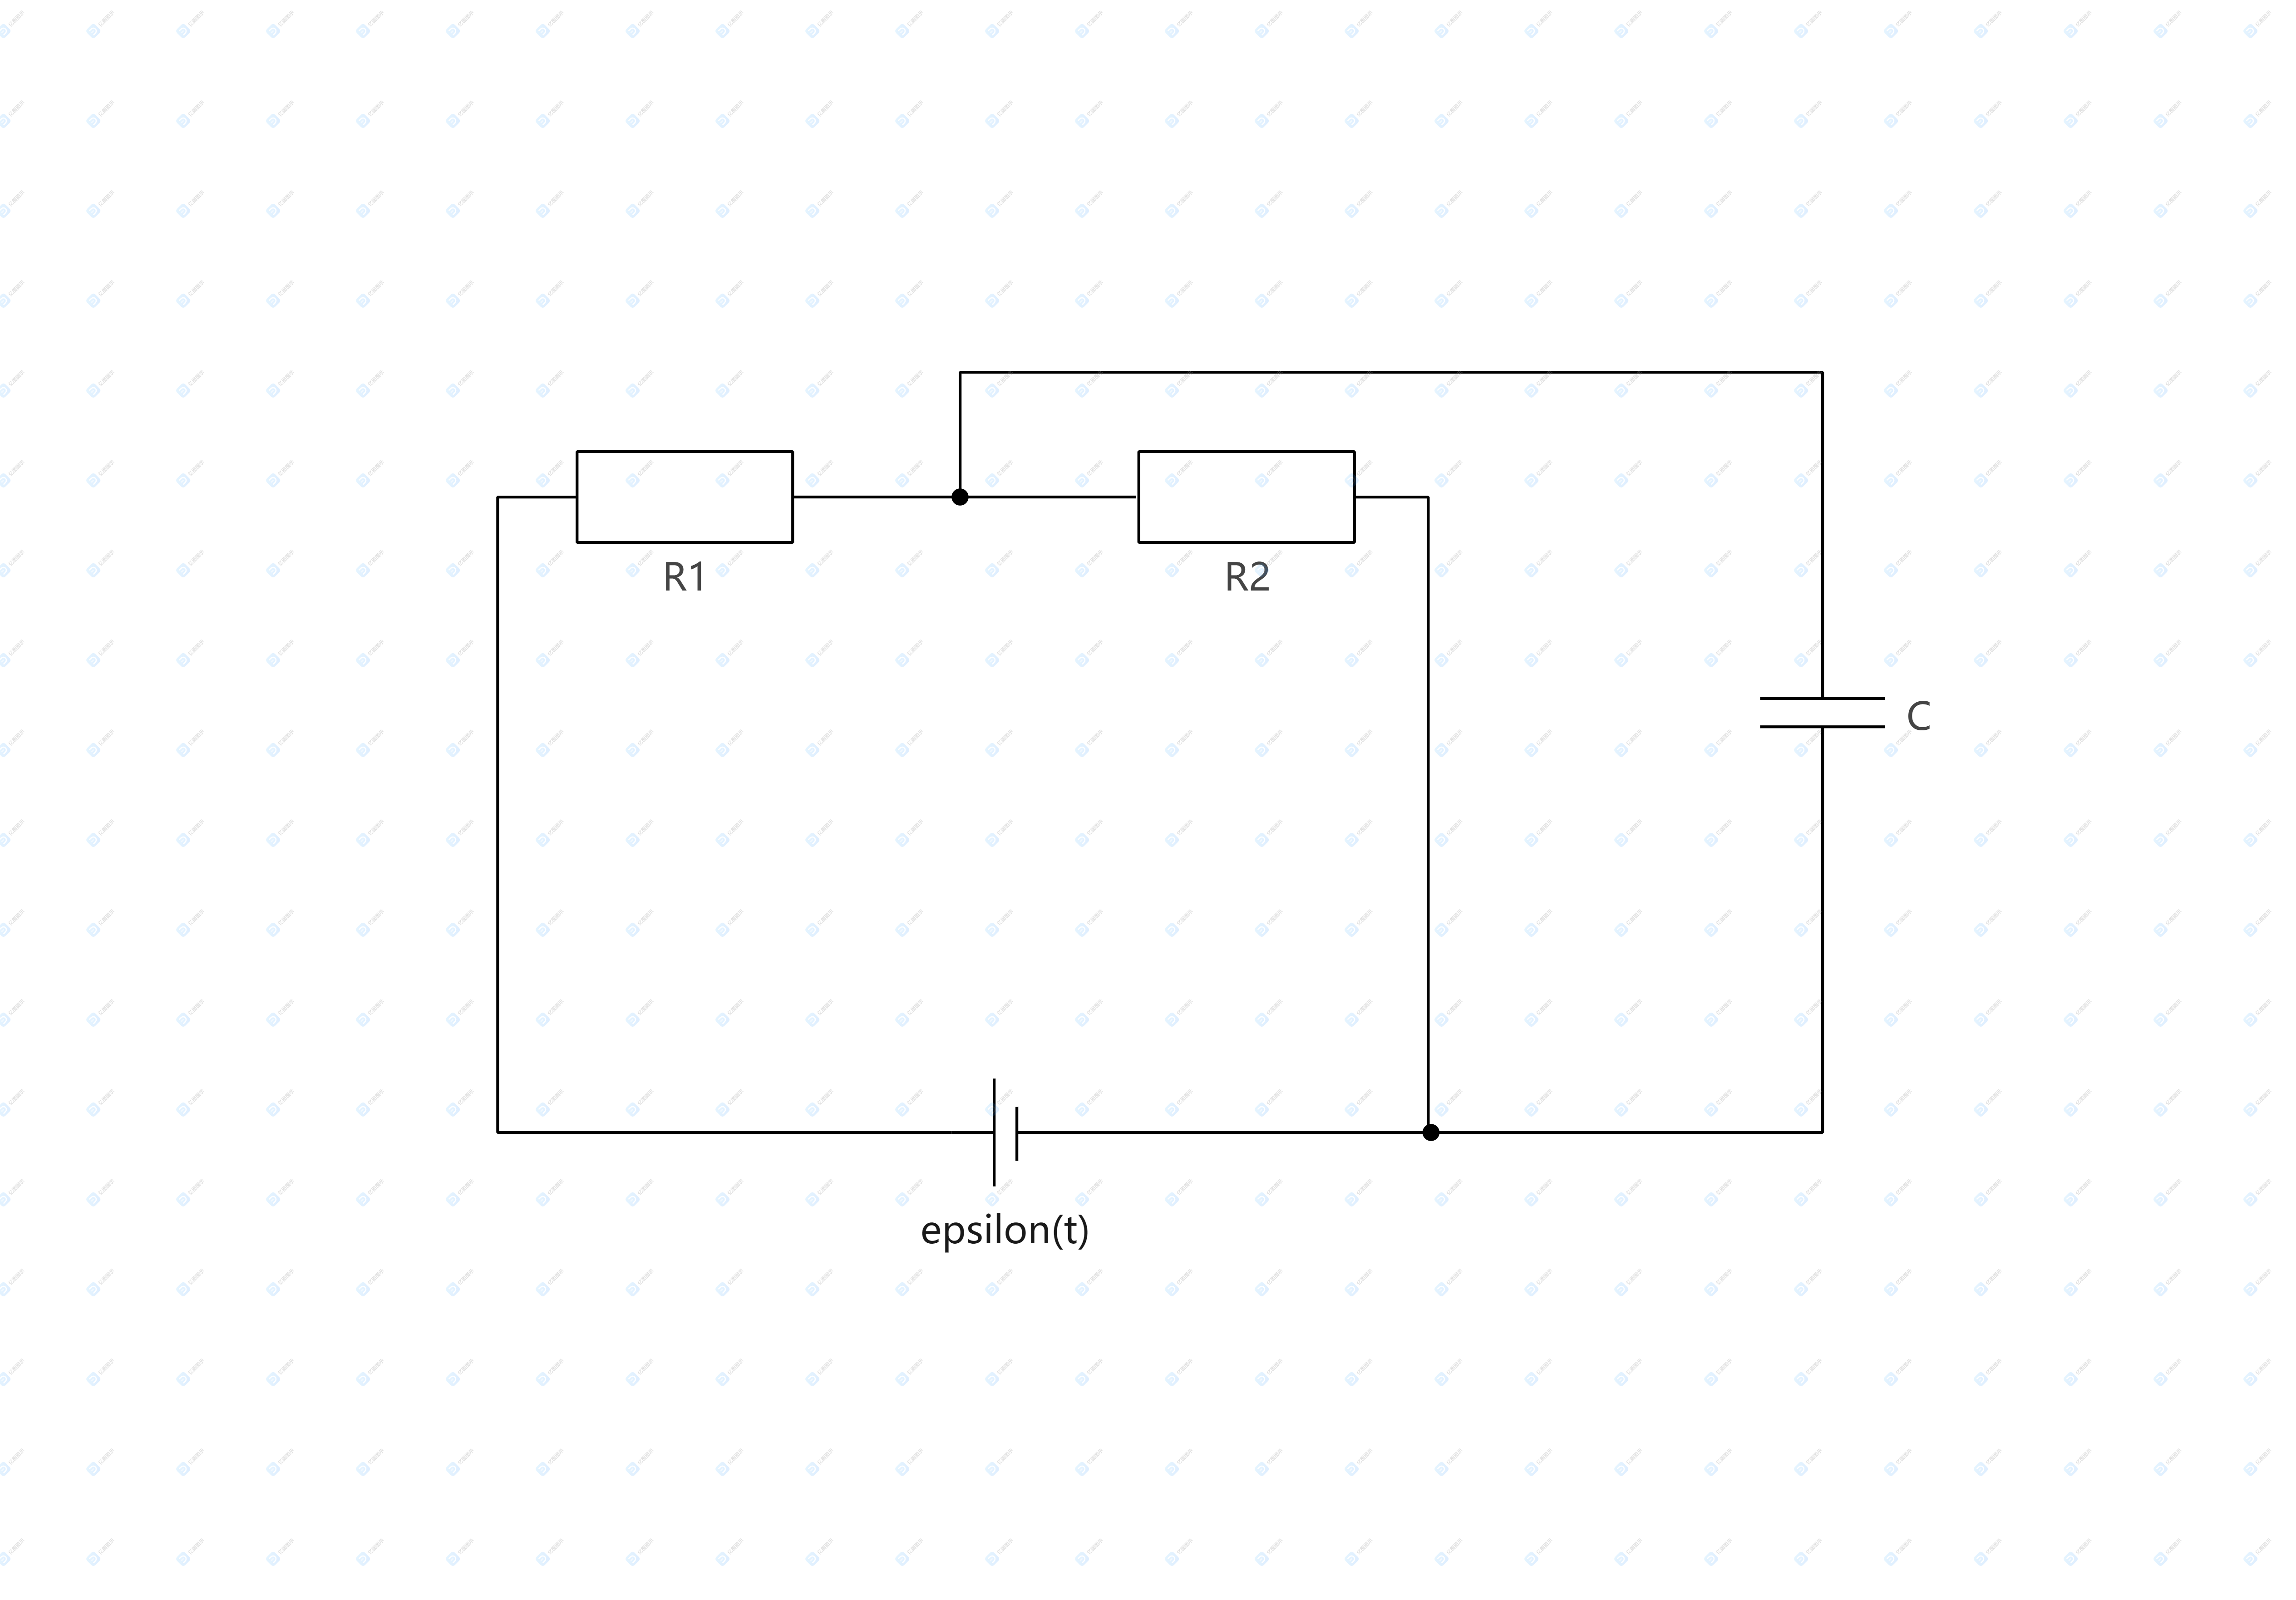
\includegraphics[scale=0.1]{c1.png}
\caption{例2电路}
\label{figure}
\end{figure}

所以,我们可以得到电容两端电压的频谱
\begin{equation}
U_c(j\omega)=E(j\omega)H(j\omega)=\frac{R_2}{R_1+R_2}\cdot[\pi\delta(\omega)+\frac{1}{j\omega}]\cdot\frac{1}{1+j\omega\tau}
\notag
\end{equation}

对其进行反傅里叶变换,就可以解得
\begin{equation}
U_c(t)=\frac{R_2}{R_1+R_2}\cdot\mathscr{F}^{-1}[\pi\delta(\omega)+\frac{1}{j\omega}-\frac{\tau}{1+j\omega\tau}]=\frac{R_2}{R_1+R_2}\cdot(1-e^{\frac{t}{\tau}})\epsilon(t)
\notag
\end{equation}

系统的无失真是指响应信号与激励信号相比,只是幅度大小和出现的时间先后不同,而无波形上的变化。可以证明,系统的无失真传输条件为:在信号的全部频带内,频率响应的幅度特性是一常数,相位特性是一通过原点的直线,这一部分要具体了解可参照教材p87。

另外,我个人认为教材p90的“调制与解调”部分比较重要,但是那些图我\sout{懒得画}不会画,所以同志们可以看一下书中这一部分的内容。

\section{连续时间信号与系统的复频域分析}
\subsection{拉普拉斯变换}
我们在使用傅里叶变换时,通常会遇到一些困难,有时函数不满足狄里赫利条件,有时函数的定义域不是实数集,所以在傅里叶变换的基础上,数学家拉普拉斯提出了拉普拉斯变换。
\begin{equation}
F(s)=\mathscr{L}[f(t)]=\int_0^{+\infty} {f(t)e^{-st}} \,{\rm d}t
\end{equation}

其中, $s=\sigma+j\omega$ 。和傅里叶反变换同理,我们也有拉普拉斯反变换。
\begin{equation}
f(t)=\mathscr{L}^{-1}[F(s)]=[\frac{1}{2\pi j}\int_{\sigma-j\infty}^{\sigma+j\infty} {F(s)e^{-st}} \,{\rm d}s]\epsilon (t)
\end{equation}

一个拉普拉斯变换对也可以表示为 $f(t)\leftrightarrow F(s)$ 。

由式(55)可知, $F(s)$ 存在的条件是被积函数收敛,从而要求满足
\begin{equation}
\lim_{t \to \infty}f(t)e^{-\sigma t}=0
\end{equation}

此即拉普拉斯变换存在的充要条件。对于函数 $f(t)$ ,若只有 $\sigma >\sigma_0$ 时,满足式(57),则称 $\sigma >\sigma_0$ 为收敛域。

可以证明,当 $f(t)\leftrightarrow F(s)$ 时,拉普拉斯变换有以下性质(此处可参考教材p128,实际上傅里叶变换和拉普拉斯变换的性质十分相似,可以结合记忆):
\begin{itemize}
\item 线性性质(不必多说)
\item 时移性质
\begin{equation}
f(t-t_0)\epsilon(t)\leftrightarrow F(s)e^{-st_0}
\end{equation}
\item 频移性质
\begin{equation}
f(t)e^{s_0 t}\leftrightarrow F(s-s_0)
\end{equation}
\item 尺度变换
\begin{equation}
f(at)\leftrightarrow \frac{1}{a}F(\frac{s}{a}), a>0
\end{equation}
\item 时域微分
\begin{equation}
\frac{{\rm d}f(t)}{{\rm d}t}\leftrightarrow sF(s)-f(0_-)
\end{equation}
\item 时域积分
\begin{equation}
\int_{0_-}^t {f(\tau)} \,{\rm d}\tau\leftrightarrow\frac{F(s)}{s}
\end{equation}
\item 复频域微分
\begin{equation}
-tf(t)\leftrightarrow \frac{{\rm d}F(s)}{{\rm d}s}
\end{equation}
\item 复频域积分
\begin{equation}
\frac{f(t)}{t}\leftrightarrow \int_s^{\infty} {F(\eta)} \,{\rm d}\eta
\end{equation}
\item 初值定理
\begin{equation}
f(0_+)\leftrightarrow \lim_{s \to \infty}sF(s)
\end{equation}
\item 终值定理,使用此定理,需满足条件: $F(s)$ 的所有极点在 $s$ 平面的左半平面内(原点处可有单阶极点)。
\begin{equation}
f(\infty)\leftrightarrow \lim_{s \to 0}sF(s)
\end{equation}
\item 时域卷积
\begin{equation}
f_1(t)*f_2(t)\leftrightarrow F_1(s)\cdot F_2(s)
\end{equation}
\item 复频域卷积
\begin{equation}
f_1(t)\cdot f_2(t)\leftrightarrow \frac{1}{2\pi j}F_1(s)*F_2(s)
\end{equation}
\end{itemize} 

可以证明下列基本拉普拉斯变换:
\begin{equation}
\epsilon(t)\leftrightarrow \frac{1}{s}
\end{equation}
\begin{equation}
\sin(\omega_0t)\leftrightarrow \frac{\omega_0}{s^2+\omega_0^2}
\end{equation}
\begin{equation}
\cos(\omega_0t)\leftrightarrow \frac{s}{s^2+\omega_0^2}
\end{equation}

通过式(61)(69),可以证明
\begin{equation}
\delta(t)\leftrightarrow 1
\end{equation}

通过频移性质,可以证明
\begin{equation}
e^{-\alpha t}\leftrightarrow \frac{1}{s+\alpha}
\end{equation}
\begin{equation}
e^{-\alpha t}\sin(\omega_0t)\leftrightarrow \frac{\omega_0}{(s+\alpha)^2+\omega_0^2}
\end{equation}
\begin{equation}
e^{-\alpha t}\cos(\omega_0t)\leftrightarrow \frac{s+\alpha}{(s+\alpha)^2+\omega_0^2}
\end{equation}

通过复频域的积分性质,可以证明
\begin{equation}
te^{-\alpha t}\leftrightarrow \frac{1}{(s+\alpha)^2}
\end{equation}
\begin{equation}
t\sin(\omega_0t)\leftrightarrow \frac{2\omega_0s}{(s^2+\omega_0^2)^2}
\end{equation}
\begin{equation}
t\cos(\omega_0t)\leftrightarrow \frac{s^2-\omega_0^2}{(s^2+\omega_0^2)^2}
\end{equation}

\subsection{拉普拉斯反变换}
一般而言,一个LTI系统的象函数是一个有理分式,所以我们重点研究有理分式的拉普拉斯反变换。若有理分式是一个假分式,我们要用长除法将其分解为一个多项式和一个真分式之和。然后,我们对这个真分式 $\frac{N_0(s)}{D(s)}$ 进行因式分解,我们对这个分式进行如下分类,并分别举例(通用公式可见教材p129)。
\begin{itemize}
\item $D(s)=0$ 的所有根均为单实根

\textbf{例3:}若 $F(s)=\frac{s-1}{s^2+3s+2}$ ,试求 $f(t)$ 。

\textbf{解:}设
\begin{equation}
F(s)=\frac{K_1}{s+1}+\frac{K_2}{s+2}
\notag
\end{equation}

因此
\begin{equation}
K_1=\left. \frac{s-1}{s+2} \right| _{s=-1}=-2
\notag
\end{equation}
\begin{equation}
K_2=\left. \frac{s-1}{s+1} \right| _{s=-2}=3
\notag
\end{equation}

由式(73)可得
\begin{equation}
f(t)=-2e^{-t}+3e^{-2t}
\notag
\end{equation}

\item $D(s)=0$ 具有共轭复根且无重复根

\textbf{例4:}若 $F(s)=\frac{s}{s^2+2s+5}$ ,试求 $f(t)$ 。

\textbf{解:}我们可以吧象函数进行如下变换:
\begin{equation}
F(s)=\frac{s+1}{(s+1)^2+2^2}-\frac{1}{2}\cdot\frac{2}{(s+1)^2+2^2}
\notag
\end{equation}

由式(74)(75)可得
\begin{equation}
f(t)=e^{-t}\cos 2t-\frac{1}{2}e^{-t}\sin 2t
\notag
\end{equation}

\item $D(s)=0$ 含有重根

\textbf{例5:}若 $F(s)=\frac{s-2}{s(s+1)^3}$ ,试求 $f(t)$ 。

\textbf{解:}将F(s)部分分式展开:
\begin{equation}
F(s)=\frac{K_{13}}{(s+1)^3}+\frac{K_{12}}{(s+1)^2}+\frac{K_{11}}{s+1}+\frac{K_2}{s}
\notag
\end{equation}

因此
\begin{equation}
K_2=\left. \frac{s-2}{(s+1)^3} \right| _{s=0}=-2
\notag
\end{equation}
\begin{equation}
K_{13}=\left. \frac{s-2}{s} \right| _{s=-1}=3
\notag
\end{equation}
\begin{equation}
K_{12}=\left. \frac{ {\rm d}}{ {\rm d}s}(\frac{s-2}{s}) \right| _{s=-1}=2
\notag
\end{equation}
\begin{equation}
K_{11}=\left. \frac{1}{2}\cdot\frac{ {\rm d}^2}{ {\rm d}s^2}(\frac{s-2}{s}) \right| _{s=-1}=2
\notag
\end{equation}

由式(63)可得
\begin{equation}
f(t)=(\frac{3}{2}t^2+2t+2)e^{-t}-2
\notag
\end{equation}
\end{itemize}

\subsection{连续时间系统的复频域分析}
现在,有了拉普拉斯变换这个强力工具,我们可以再把例1做一遍。

\textbf{解:}将方程两边进行拉普拉斯变换,得:
\begin{equation}
sR(s)-2+2R(s)=E(s)
\notag
\end{equation}

整理后得:
\begin{equation}
R(s)=\frac{2}{s+2}+\frac{E(s)}{s+2}
\notag
\end{equation}

$\frac{1}{s+2}$ 被称为系统函数 $H(s)$ ,它与系统的激励无关,只取决于系统本身的特性。可以证明,上式的第一项时零输入响应,第二项为零状态响应。将 $E(s)=1/s$ 代入,得:
\begin{equation}
R(s)=\frac{3}{2}\cdot\frac{1}{s+2}+\frac{1}{2s}
\notag
\end{equation}

对 $R(s)$ 进行拉普拉斯反变换,解得系统的全响应。
\begin{equation}
r(t)=\frac{3}{2}e^{-2t}+\frac{1}{2}\quad(t>0)
\notag
\end{equation}

由此,我们得到了求LTI响应的第四种方法:拉普拉斯变换法。这种方法比上面三种方法都要简单,但是要求激励必须从零开始。其步骤如下:
\begin{itemize}
\item 将微分方程两边进行拉普拉斯变换。
\item 求得 $R(s)$ 。
\item 用拉普拉斯反变换解得全响应。
\end{itemize} 

在上一章,我们做到了利用傅里叶变换求电路的零状态响应。现在有了拉普拉斯变换这个工具,我们可以更进一步,求出线性电路的全响应,这里介绍一下电路元件的 $s$ 域模型。

电阻、电感和电容的时域关系分别为
\begin{equation}
u_R(t)=Ri_R(t)
\end{equation}
\begin{equation}
u_L(t)=L\frac{{\rm d}i_L(t)}{{\rm d}t}
\end{equation}
\begin{equation}
u_C(t)=\frac{1}{C}\int_{-\infty}^t {i_C(\tau)} \,{\rm d}\tau
\end{equation}

将以上三式进行拉普拉斯变换,得
\begin{equation}
U_R(s)=RI_R(s)
\end{equation}
\begin{equation}
U_L(s)=sLI_L(s)-Li_L(0_-)
\end{equation}
\begin{equation}
U_C(s)=\frac{1}{sC}I_C(s)+\frac{1}{s}u_C(0_-)
\end{equation}

这便是s域元件的串联模型,图3是其具象化。
\begin{figure}[htbp]
\centering
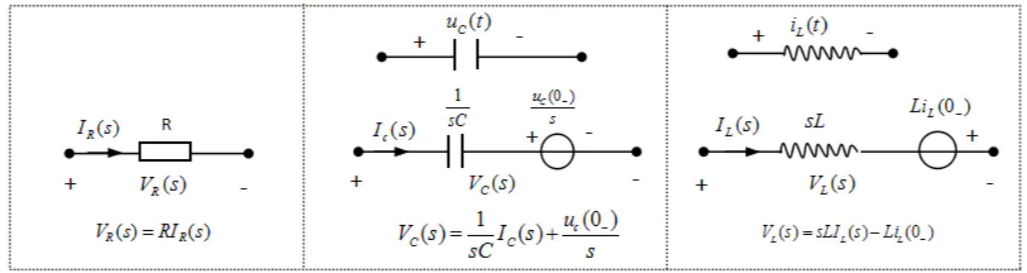
\includegraphics[scale=0.6]{p2.png}
\caption{s域原件串联模型}
\end{figure}

我们亦可以改写以上三式
\begin{equation}
I_R(s)=\frac{1}{R}U_R(s)
\end{equation}
\begin{equation}
I_L(s)=\frac{1}{sL}U_L(s)+\frac{1}{s}i_L(0_-)
\end{equation}
\begin{equation}
I_C(s)=sCU_C(s)-Cu_C(0_-)
\end{equation}

这就是s域元件的并联模型,这里举一个例子进一步说明。

\begin{figure}[htbp]
\centering
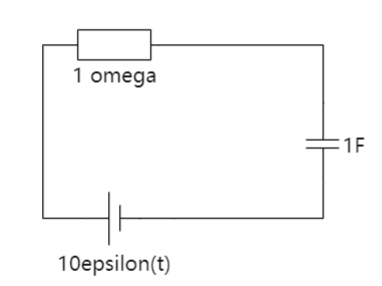
\includegraphics{p4.png}
\caption{例6电路图}
\end{figure}

\textbf{例6:}如图4,已知 $e(t)=10\epsilon(t), C=1F, R=1\Omega, U_C(0_-)=5V$ ,求 $u_C(t)$ 。

\textbf{解:}首先画出零输入时的s域图,如图5。
\begin{figure}[htbp]
\centering
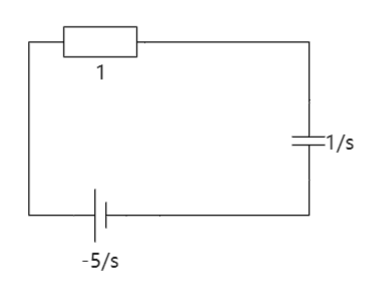
\includegraphics{p5.png}
\caption{零输入s域图}
\end{figure}

因此
\begin{equation}
R_{zi}(s)=\frac{5}{s}\cdot\frac{1}{1+\frac{1}{s}}=\frac{5}{s+1}
\notag
\end{equation}
\begin{equation}
r_{zi}(t)=5e^{-t}
\notag
\end{equation}

再画出零状态时的s域图,如图6。
\begin{figure}[htbp]
\centering
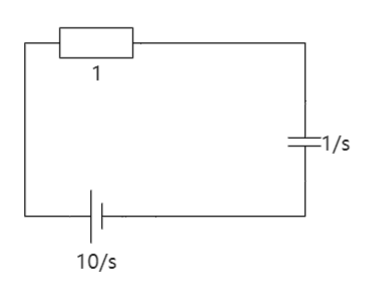
\includegraphics{p6.png}
\caption{零状态s域图}
\end{figure}

因此
\begin{equation}
R_{zs}(s)=\frac{10}{s}\cdot\frac{\frac{1}{s}}{1+\frac{1}{s}}=10(\frac{1}{s}-\frac{1}{s+1})
\notag
\end{equation}
\begin{equation}
r_{zs}(t)=10-10e^{-t}
\notag
\end{equation}

解得全响应
\begin{equation}
r(t)=r_{zi}(t)+r_{zs}(t)=10-5e^{-t}
\notag
\end{equation}

\subsection{系统函数的零、极点分布}
我们知道,LTI系统的系统函数 $H(s)=N(s)/D(s)$ 是一个有理分式。我们称 $D(s)=0$ 的根为系统函数的极点,$N(s)=0$ 的根为系统函数的零点。将系统函数的零、极点表在 $s$ 平面上,并用圆圈表示零点,叉表示极点,这个图成为系统函数的零极图。图7就是一些系统函数的零极图。
\begin{figure}[htbp]
\centering
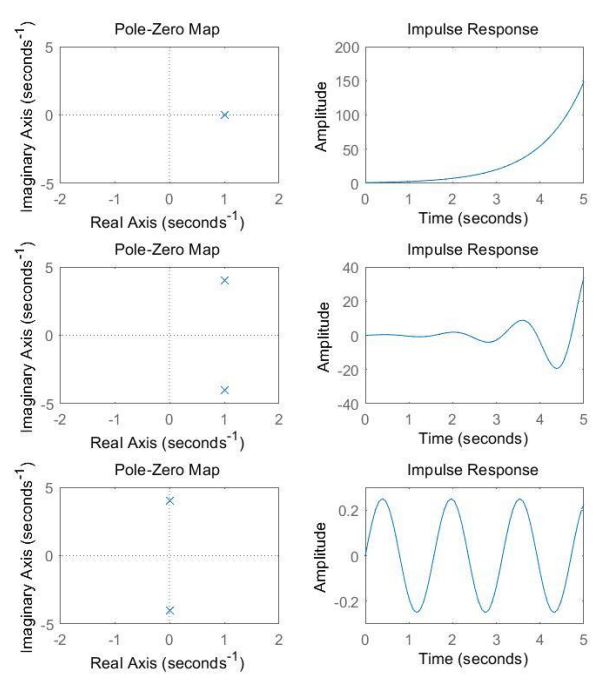
\includegraphics[scale=0.9]{p7.png}
\caption{一些系统的零极图}
\end{figure}

我们可以通过零极点的分布情况来推出冲激响应 $h(t)$ 的函数形式,在此讨论单极点情况:
\begin{itemize}
\item 极点再纵轴上:若在原点上,则冲激响应为阶跃函数;若在虚轴上,则冲激响应为等幅振荡。
\item 极点再纵轴左侧:若在实轴上,则冲激响应为单调衰减指数函数;若不在实轴上,则冲激响应为减幅振荡。
\item 极点再纵轴右侧:若在实轴上,则冲激响应为单调增长指数函数;若不在实轴上,则冲激响应为增幅振荡。
\end{itemize} 

除了以上知识点,我认为本章的“连续时间系统s域模拟”(教材p155)和“系统的稳定性”(教材p159)也是比较重要的知识点,因为我\sout{懒得画}不会画,所以同志们可以看一下书中这一部分的内容。
\end{document}
